\documentclass[12pt]{article}
\usepackage{amsmath}
\usepackage{amssymb}
\usepackage{tikz}
\usepackage{circuitikz}
\usepackage{tkz-euclide}
\usepackage{pgfplots}
\usepackage{siunitx}
\usepackage[many]{tcolorbox}
\pgfplotsset{compat=1.18}
\newtcolorbox{BOX}{
colframe=white,
colback=white,
enhanced,
boxrule=1.5pt,
borderline={0.75pt}{0pt}{dashed},
}
\tikzset{european}
\title{Preparation Tests}
\author{Hertzberg, Joakim D.}
\date{\today}

%END OF PREAMBLE
\begin{document}
\maketitle
\begin{center}
FYS01a: Physics 1a
\vfill
This document uses \LaTeX\ in combination with \emph{TikZ} for typesetting.
\end{center}
\newpage
\tableofcontents
\newpage
\section{ }
\textbf{a)} \bigbreak

$$F = \left\{ \begin{array}{l}
		||F|| = 15 \unit{N} \\
		\theta_F=45^{\circ}
		\end{array} \right.$$

	$$\dot{v} = 0 \implies F_x = -F_f$$

	$$\vec{F} = \begin{pmatrix} 15\cos{\theta} \\ 15\sin{\theta} \end{pmatrix}$$
	$$\vec{F_x} = -\vec{F_f} \implies \vec{F_f} = 
	-\begin{pmatrix} 0 \\ 15\cos{\theta} \end{pmatrix} 
	\approx \begin{pmatrix} 0 \\ -10.6067N \end{pmatrix}$$

 
\textbf{b)} \bigbreak
Assume $g=9.82$. \bigbreak
$$\vec{F_N} = \Sigma \vec{F_y} = \vec{F_g} + \vec{F_y}$$
$$\vec{F_N} = \begin{pmatrix} 0 \\ 5 \times -9.82 \end{pmatrix} + \begin{pmatrix} 0 \\ 15\sin{45^{\circ}} \end{pmatrix}$$
$$\vec{F_N} \approx \begin{pmatrix} 0 \\ -38.493 \end{pmatrix}N$$

\section{ }
\newpage
\section{ }
Here, it is stated that $300N$ are required to lift a stone upwards. This means that $300$ is just at the threshold where $\dot{v} > 0$. \\
That means that we are at a place where $\dot{v} = 0 + \frac{1}{\infty}$. This is however unsolvable, let's write it as such instead: 
$$\lim_{x\rightarrow0} \left( \dot{v} = x \right)$$

$$\lim_{x\rightarrow0} \left( x = \frac{\begin{pmatrix} 0 \\ 300 \end{pmatrix}}{m} - \begin{pmatrix} 0 \\ -9.82 \end{pmatrix} \right)$$
$$\lim_{x\rightarrow0} \left( x = \begin{pmatrix} 0 \\ \frac{300}{m} - 9.82 \end{pmatrix} \right)$$
$$\lim_{x\rightarrow0} \left( x = \frac{300}{m}-9.82 \right)$$
$$\lim_{x\rightarrow0} \left( m(x+9.82) = 300 \right)$$
$$\lim_{x\rightarrow0} \left( m = \frac{300}{x+9.82}\right)$$
$$m = \frac{300}{0+9.82}$$
$$m = \frac{300}{9.82}$$
$$m \approx 30.550 \ \unit{Kg}$$

\section{ }
Assuming the center of mass is at equal distance from both arms and $g=9.82 \unit{m.s^{-2}}$: 
$$\vec{F_g} = \begin{pmatrix} 0 \\ -9.82*53 \end{pmatrix} = \begin{pmatrix} 0 \\ -520.6 \end{pmatrix}$$
$$F_arm = \frac{||F_g||}{2} = \frac{520.6}{2}=260.23 \unit{N}$$

\section{ }

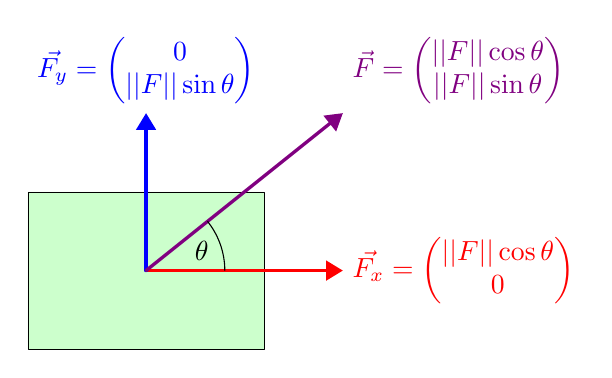
\begin{tikzpicture}
\tkzDefPoint(0,0){A}
\tkzDefPoint(3,0){B}
\tkzDefPoint(3,2){C}
\tkzDefPoint(0,2){D}
\tkzDefPoint(1.5,1){E}
\tkzDefPoint(4,1){F}
\tkzDefPoint(1.5,3){G}
\tkzDefPoint(4,3){H}
\tkzDrawPolygon[fill=green!20!white](A,B,C,D)
\tkzDrawSegment[-Triangle,color=red,very thick](E,F)
\tkzDrawSegment[-Triangle,color=blue,very thick](E,G)
\tkzDrawSegment[-Triangle,color=blue!50!red,very thick](E,H)
\node[right, red] at(F) {$\vec{F_x} = \begin{pmatrix} ||F||\cos{\theta} \\ 0 \end{pmatrix}$};
\node[above, blue] at(G) {$\vec{F_y} = \begin{pmatrix} 0 \\ ||F||\sin{\theta}\end{pmatrix}$};
\node[above right, blue!50!red] at(H) {$\vec{F} = \begin{pmatrix} ||F||\cos{\theta} \\ ||F||\sin{\theta} \end{pmatrix}$};
\tkzMarkAngle(F,E,H)
\tkzLabelAngle[pos=0.75](F,E,H){$\theta$}

\end{tikzpicture}

\end{document}
